This layer is for communication between the control layer and the UR5 layer in details. It have a router as its subsystem.

\begin{figure}[h!]
	\centering
 	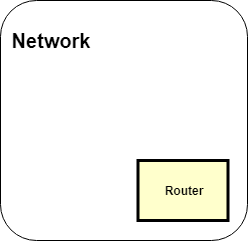
\includegraphics[width=0.60\textwidth]{images/Network_Layer}
 \caption{Network layer diagram}
\end{figure}

\subsection{Router}
The router is use as a mean of communication to the UR5.

\subsubsection{Assumptions}
The IP address is given and known to the UR5 through the polyscope.

\subsubsection{Responsibilities}
The router gives an IP address that allow the software to send instructions to the UR5.

\subsubsection{Subsystem Interfaces}
There is two interfaces connecting to the router.

\begin {table}[H]
\caption {Router interfaces} 
\begin{center}
    \begin{tabular}{ | p{1cm} | p{6cm} | p{3cm} | p{3cm} |}
    \hline
    ID & Description & Inputs & Outputs \\ \hline
    \#xx & Control Box & \pbox{3cm}{N/A} & \pbox{3cm}{UR Script(UR Instructions)}  \\ \hline
    \#xx & Raspbery Pi & \pbox{3cm}{UR Script(UR Instructions)} & \pbox{3cm}{N/A}  \\ \hline
    \end{tabular}
\end{center}
\end{table}

